\documentclass[12pt]{article}
\raggedbottom

\usepackage[utf8]{inputenc}
\usepackage{graphicx}
\usepackage[english]{babel}
\usepackage{csquotes}
\usepackage{lipsum}
\usepackage{fancyhdr}
\usepackage{pdfpages}
\usepackage{wrapfig}
\usepackage{siunitx}
\usepackage{subcaption}
\usepackage{float}
\usepackage{enumitem}
\usepackage{subcaption}
\usepackage{framed}
\usepackage{listings,xcolor}
\usepackage{inconsolata}
\usepackage{setspace}
\usepackage[T1]{fontenc}
\usepackage[hidelinks]{hyperref}
\usepackage{booktabs}
\usepackage{amsmath}
\usepackage{csquotes}
\usepackage[backend=biber, sorting=none]{biblatex}
\usepackage[a4paper,width=160mm,top=25mm,bottom=25mm]{geometry}

\captionsetup{compatibility=false}
\definecolor{shadecolor}{gray}{0.8}
%\nocite{*}
\addbibresource{sources.bib}
\setcounter{biburllcpenalty}{7000}
\setcounter{biburlucpenalty}{8000}

\title{\textbf{\textsc{Assignment 2: File System}}\\Digital Forensics}

\author{Elisa Pioldi\\
        ID 12305812}
\date{November 28, 2023}

\begin{document}

\maketitle

\section{Factual part}

\subsection{Background}

The company Indiga has developed a video game called Snipper, but the designer Sabrina found that the main character of the brand new game presented by competing company was suspiciously similar to her own concept.
The investigators have confiscated the home computer of Peter (who is a developer at Indiga) and have acquired a forensic image. 
Hash (SHA-1) of the image is \texttt{b4c3ae80f840bb612f982ba5081872b8a6a19e83}.

The goal is to find evidence that Peter has leaked information about the game to the competing company.

The Indiga employees involved in the case are the following:
\begin{itemize}
    \item \textbf{Anna}: director and founder of Indiga, mainly responsible for business challenges
    \item \textbf{John}: co-director, founder and lead developer
    \item \textbf{Iris}: developer
    \item \textbf{Peter}: developer and primary suspect
    \item \textbf{Sabrina}: designer
\end{itemize}

\subsection{Software and hardware specifications}
\label{sec:specs}

For this analysis, I utilized the following software:

\begin{itemize}
    \item \textbf{Autopsy} \cite{autopsy} -- version 1.24 (update 7); to perform container mounting and access.
    \item \textbf{Qemu} \cite{qemu}; to convert the image from qcow format to raw format.
    \item \textbf{PhotoRec} \cite{photorec} -- version 6.2.6; to perform file carving. 
    \item \textbf{TeslaDecrypter} \cite{tesla-decrypt}; to decrypt the files encrypted by the ransomware TeslaCrypt.
\end{itemize}

\begin{figure}[!ht]
    \centering
    \begin{subfigure}[b]{0.3\textwidth}
        \centering
        
\includegraphics[width=\textwidth]{images/autopsy.png}.
        \caption{Autopsy logo.}
        \label{fig:autopsy}
    \end{subfigure}
    \hspace{30 pt}
    \begin{subfigure}[b]{0.3\textwidth}
        \centering
        
\includegraphics[width=\textwidth]{images/photorec.png}.
        \caption{PhotoRec logo.}
    \label{fig:photorec}
    \end{subfigure}
\end{figure}

\subsection{Initial setup}

First, I had to convert the image from qcow format to raw format, which is supported by the utilized tool, using Qemu.

Then, I analized the image using Autopsy. After a first analysis, I performed file carving using PhotoRec on the unallocated space of the image.

\subsection{System specifications}

The image analyzed is a desktop computer, with a 64-bit architecture, running Windows 7 Professional Service Pack 1. 
You can find more details in Table \ref{table:stats} (please notice that as `last time the system was running' I considered the last time there was a system event).

\begin{table}[!ht]
    \centering
    \begin{tabular}{ll}
    \toprule
        \multicolumn{2}{c}{\textbf{System specifications}} \\
        \midrule
        \textbf{Operating system} & Windows 7 Professional Service Pack 1 \\
        \textbf{Computer name} & HYRULE \\
        \textbf{Installing date of the OS} & 2016-07-06 23:27:42 GMT+0000 \\
        \textbf{Last time the system was running} & 2016-09-05 15:28:53 CEST \\
        \textbf{SID} & S-1-5-21-3032217210-630098460-752710606-1001 \\
    \bottomrule
    \end{tabular}
    \caption{Statistics of some cracked containers.}
    \label{table:stats}
\end{table}

\subsection{Suspicious activity}

After a deep analysis of the file system, I found numerous files linked to tutorials about games and game design, with a lot of examples of concept arts. 

Moreover, analyzing web history, I found out that Peter has visited numerous websites to find a way to hide files on his computer. 

\subsection{Notable files}

In this analysis I will focus on the files that I found more relevant to the case, which are two e-mail exchanges and a photo of a concept art.

To verify the integrity of files found, I computed the SHA-1 checksum of them. The results are shown in Table \ref{table:sha1}.

The major evidence that I found is the following e-mail exchanges between Peter and Iris.

\subsubsection{Email exchanges}

\paragraph{First email exchange}
\label{sec:first-mail}

The following e-mail exchange is the first one in time between Peter and Iris, where they are planning a date.

\begin{shaded}
\begin{verbatim}
> Am Wed, 24 Aug 2016 00:48:30 +0200
> schrieb briennefan@openmailbox.org:
>> Hihi
>> 
>> Hi Peter, now we can chat. ;)

On 2016-08-24 01:28, Peter wrote:
> Hey,
> 
> nice! Puh the traffic today was terrible...
> Hope you had a nice ride. :)
> 
> Am Wed, 24 Aug 2016 00:48:30 +0200
> schrieb briennefan@openmailbox.org:

Yeah no problem at all.
Say, do you want to go for a drink someday? ;)
\end{verbatim}
\end{shaded}

\paragraph{Second email exchange}
The following e-mail exchange is the second one in time between Peter and Iris, where they are talking about a date they had.

\begin{shaded}
\begin{verbatim}
On 2016-08-24 01:36, Peter wrote:
> Hey,
> 
> it felt like one, hope do not take it wrong, that I call our meeting a
> date.

I'm ok with that :)
I also think, that it was a date :)

But it should be a thing between us two and we should keep it as a 
secret at work. ;)
\end{verbatim}
\end{shaded}

\paragraph{Third email exchange}
The following e-mail exchange is the third one in time between Peter and Iris, where Iris is asking Peter about some design concepts of Sabrina.

\begin{shaded}
\begin{verbatim}
> >> > On 2016-08-24 01:43:05 +0200
> >> > schrieb briennefan@openmailbox.org:
> >> >> Hey, can you do me a favor?
> >> >> you seen some design concepts of Sabrina?

> >> On 2016-08-24 01:45, Peter wrote:
> >> > Nope, not really. She only shows it to Anna and John, but I know
> >> > that she keeps it in her desk. Why?

> > On 2016-08-24 01:46:58 +0200
> > schrieb briennefan@openmailbox.org:
> >> Can you get a copy for me? I'm very interested in it :)

> On 2016-08-24 01:49, Peter wrote:
> > Hehe why don't you just wait until she presents the first 3D model?
> > Sometimes she lets her drawings unlocked on her table, but I don't
> > think that I should copy them :/

On 2016-08-24 01:51:15 +0200
schrieb briennefan@openmailbox.org:
> I'm very impatient. Please do it for me, maybe I will reward you with 
> another date? ;)

Uhm ok, I'll look what I can do for you :)
\end{verbatim}
\end{shaded}

\paragraph{Fourth email exchange}
This is the last e-mail exchange between Peter and Iris, where Peter is asking Iris about the leak of information.

\begin{shaded}
\begin{verbatim}
Date: Wed, 24 Aug 2016 02:01:36 +0200
From: Peter <peter1983@openmailbox.org>
To: briennefan@openmailbox.org
Subject: Question

Hey Iris!
Anna and john asked me today, if I leaked some information about our
work. I denied everything, I don't want you to get into trouble. What
have you done with the desired item from Sabrina. Please answer me
Iris, I don't want to discuss this at Work.

Peter
\end{verbatim}
\end{shaded}
For further analysis on the mail exchange, see Section \ref{sec:mail}.

\subsubsection{Concept art}

I found a photo of a concept art, which is shown in Figure \ref{fig:nina}.
This file was found in 3 different situations: one as deleted file, one as encrypted file (see Section \ref{sec:malware}) and only the last one as a normal file which could be opened.

Analysis of the picture is shown in Section \ref{sec:art}.

\begin{figure}[!ht]
    \centering
    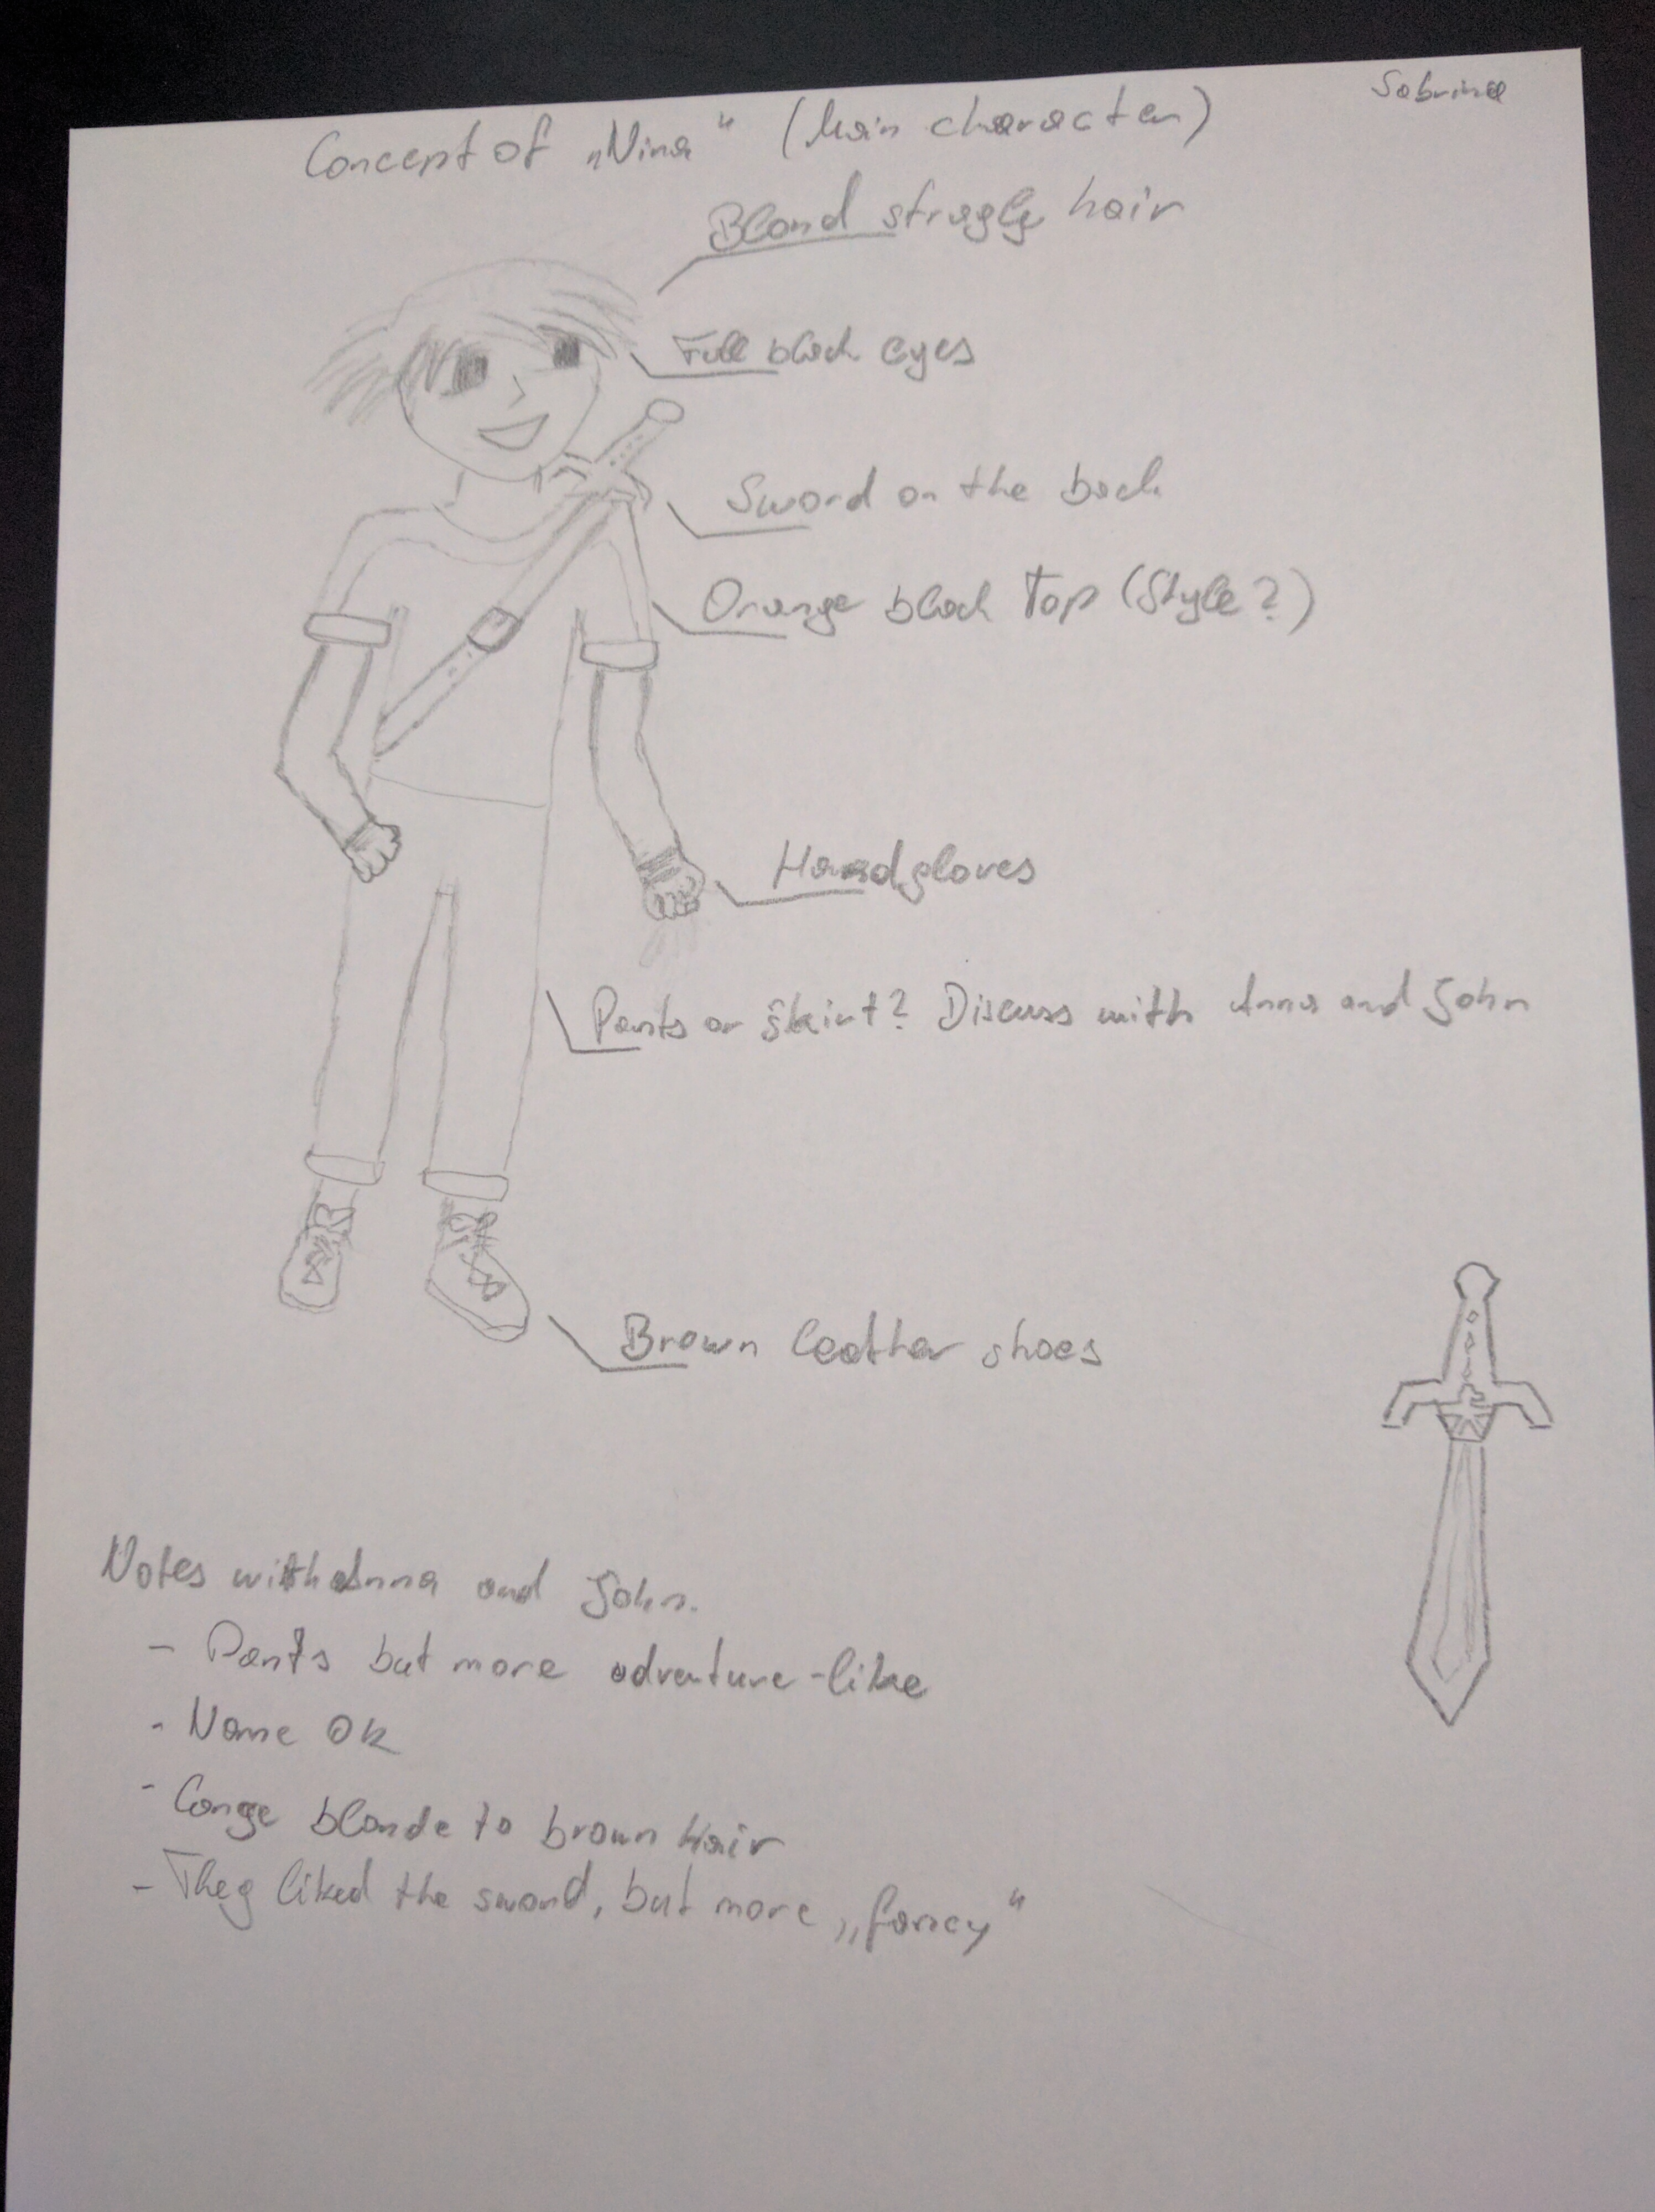
\includegraphics[width=\textwidth]{images/nina_concept.jpg}
    \caption{Nina concept art.}
    \label{fig:nina}
\end{figure}

\begin{table}[!ht]
    \centering
    \begin{tabular}{ll}
    \toprule
        \textbf{Content} & \textbf{SHA-1} \\
        \midrule
        Nina concept art \\(IMG\_20160823\_130922.jpg) & \texttt{98296EF2B0A297A323EA36CA7E5C31399D412D91} \\
        1st email exchange with Iris (4) & \texttt{7CCB4BF11E4601E9DCFC1821F286CF673DA4142E} \\
        2nd email exchange with Iris (6) & \texttt{74D1A62DCB6332BD1215083B99FB0A92F95CDDE4} \\
        3rd email exchange with Iris (8) & \texttt{3486BE7A44BA05D0EED985881C38C2DC226CC4E5} \\
        4th email exchange with Iris (11) & \texttt{E08A6FCED0D464E55C4C4357164B4258E9F634B9} \\
    \bottomrule
    \end{tabular}
    \caption{Checksums of the most important files for evidence.}
    \label{table:sha1}
\end{table}

\subsection{Malware traces}

In addition of the files mentioned above, I found a great amount of files with the extension \texttt{.mp3}, which were all encrypted. They were in different location, but all of them were in private folders of Peter and looked like personal files.
The files mentioned are the following (see Table \ref{table:sha1-malware} for the checksums):
\begin{itemize} 
    \itemsep-0.5em 
    \item \texttt{Fallen\_Champions\_concept\_art\_3.jpg.mp3}
    \item \texttt{Fungus-Documentation.pdf.mp3}
    \item \texttt{IMG\_20160823\_130922.jpg.mp3}
    \item \texttt{Leonard\_Nimoy\_William\_Shatner\_Star\_Trek\_1968.JPG.mp3}
    \item \texttt{monster\_concept\_art\_vii\_by\_d\_faultx.jpg.mp3}
    \item \texttt{myrating.csv.mp3}
    \item \texttt{passwords.docx.mp3}
    \item \texttt{unityassetstoreguide.pdf.mp3}
    \item \texttt{contactdata.csv.mp3}
\end{itemize}

\begin{table}[!ht]
    \centering
    \begin{tabular}{ll}
    \toprule
    \textbf{Content} & \textbf{SHA-1} \\
    \midrule
    \texttt{Fallen\_Champions\_concept\_art\_3} & \texttt{457598C7417C909EEA12756E8DA5775311627B36} \\
    \texttt{Fungus-Documentation} & \texttt{DE51A21FBF86F8A840F9E44FB9CCB1986B31ECFD} \\
    \texttt{IMG\_20160823\_130922} & \texttt{98296EF2B0A297A323EA36CA7E5C31399D412D91} \\
    \texttt{Leonard\_Nimoy\_William\textelp{}} & \texttt{E02A76764D9DF6EACA8A237A74E1A5E6EC35C356} \\
    \texttt{monster\_concept\_art\_vii\textelp{}} & \texttt{6BB17DAF3AF58C660D50C47D2CA0CB0A0F32BD96} \\
    \texttt{myrating} & \texttt{8C08911E7C740AC2A4E15F876DACFE7C4846D2DE} \\
    \texttt{passwords} & \texttt{11473175A82EF96BF0588BFC5308FD787A7FC17F} \\
    \texttt{unityassetstoreguide} & \texttt{A6BDBA728EBC450CE7353596C460543094DC5196} \\
    \texttt{contactdata3} & \texttt{AD862FCC026E81639E15033DD886EC09CB46CB14} \\
    \bottomrule
    \end{tabular}
    \caption{Checksums of the files encrypted by the malware.}
    \label{table:sha1-malware}
\end{table}

As confirmation of this anomaly, I found an e-mail from Peter to tech support, signaling this weird behavior of the computer:

\begin{shaded}
\begin{verbatim}
Hello Dude!

Can you help me? Suddenly my files changed to mp3's and I got some
strange messages with "IMPORTANT INFORMATION" and I cannot open those
files... I did nothing great, I browsed the web for stuff and then I
got this message...
Maybe you can help me? I got some of the data back, but I saved the mp3
to be safe.

Thank you
Peter
\end{verbatim}
\end{shaded}

I also found three files called \texttt{\_RECoVERY\_+wdbic} of different types (PNG, HTML, TXT) in the \texttt{Roaming} directory. You can see the content of the HTML file in Figure \ref{fig:rec-file}. Moreover, I found a suspicious JavaScript script in the cache of the browser.

You can see Table \ref{table:sha1-malware-info} for the checksums of the files mentioned above.

\begin{figure}[!ht]
    \centering
    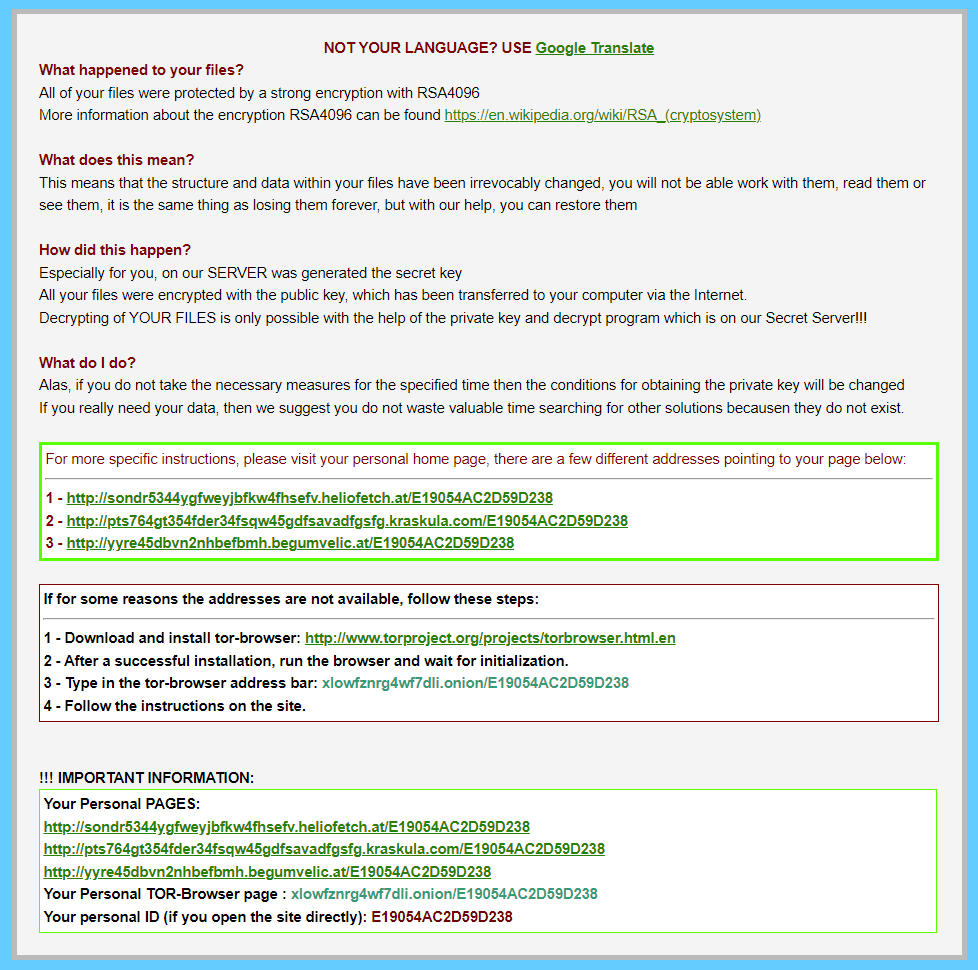
\includegraphics[width=\textwidth]{images/recovery_file.png}
    \caption{Ransomware note.}
    \label{fig:rec-file}
\end{figure}
Further analysis on these files is shown in Section \ref{sec:malware}.

\begin{table}[!ht]
    \centering
    \begin{tabular}{ll}
    \toprule
    \textbf{Content} & \textbf{SHA-1} \\
    \midrule
    Email exchange with the tech support (12) & \texttt{A9E2290731742703465F183C5F4E52CD640E65C6} \\
    \texttt{\_RECoVERY\_+wdbic.html} & \texttt{FD47F9BC079230331F239A6DE549FB60F625E124} \\
    \texttt{\_RECoVERY\_+wdbic.png} & \texttt{8BDAF44B3454C4DE35B13F66AB04F8092DCAFBE5} \\
    \texttt{Suspicious JS script} & \texttt{7A34E731F9D94317C715AA211387E6C207CA34E3} \\
    \bottomrule
    \end{tabular}
    \caption{Checksums of the ransomware notes and the e-mail to tech support.}
    \label{table:sha1-malware-info}
\end{table}

\section{Expert testimony}

\subsection{Mail exchange}
\label{sec:mail}

Reading the e-mails, I found out that Iris has asked Peter to steal the concept art from Sabrina's desk (since sometimes she leaves drawings unlocked on the table), getting advantage of the fact that Peter seems to like her: from previous e-mails (first and second exchange), I understood that they have been already on a date.

From the fourth e-mail exchange, I found out that Peter has been accused of leaking information about the game, and he is asking Iris to talk about it in private.

These two emails are the evidence that Iris has leaked information about the game to the competing company with high probability, getting advantage of the fact that Peter likes her.

\subsection{Concept art}
\label{sec:art}

The concept art found is a drawing of the main character of the game, Nina. We can spot the name of the designer, Sabrina, on the top right corner of the image and the mentions to Anna and John, who suggested some changes to the design. This is probably the file that Iris asked Peter to steal.

\subsection{Malware}
\label{sec:malware}

\subsubsection{Discovery}
I found traces on the device of the malware TeslaCrypt, which is a ransomware that encrypts files on the victim's computer and asks for a ransom to decrypt them \cite{teslacrypt}.
The first thing I noticed was the great amount of files with the extension \texttt{.mp3}, and the fact that they were all encrypted.
Moreover, I found an e-mail from Peter to tech support, signaling this weird behavior of the computer.

Conducting a search on the Internet, I found out that the malware TeslaCrypt is responsible for this kind of encryption. This malware is common downloading games: this is compatible with the fact that Peter is close to the gaming industry and seems to be a videogame lover. I also found in the cache of the browser some suspicious JavaScript scripts that were probably used to download the malware, since there are references to websites that are known to be used maliciously.

I started looking for the ransom note, which is usually a file with the recovery instructions: indeed I found the file \texttt{\_RECoVERY\_+wdbic.html} (see Figure \ref{fig:rec-file}).

\subsubsection{Decryption}
Conducting some researches, I found out that the author of the ransomware have released the master key \cite{teslacrypt-masterkey}: \\
\texttt{440A241DD80FCC5664E861989DB716E08CE627D8D40C7EA360AE855C727A49EE}

There are some tools to decrypt the files: I used the tool TeslaDecrypter \cite{tesla-decrypt} to decrypt the files with the extension \texttt{.mp3}.

One of the file affected was the concept art of the game.

\subsection{Future work}

After this analysis, I would recommend to the investigators to analyze the computer of Iris, to find out if she has leaked the concept art sent by Peter. It would be significant to analyze her e-mails and her web history, to find out if she has any contact with the competing company.

\addcontentsline{toc}{chapter}{References}
\printbibliography[title={References}]

\end{document}